\documentclass{standalone}
\usepackage{pgfplots}
\pgfplotsset{compat=1.17}
\usepackage{amsmath}

\begin{document}

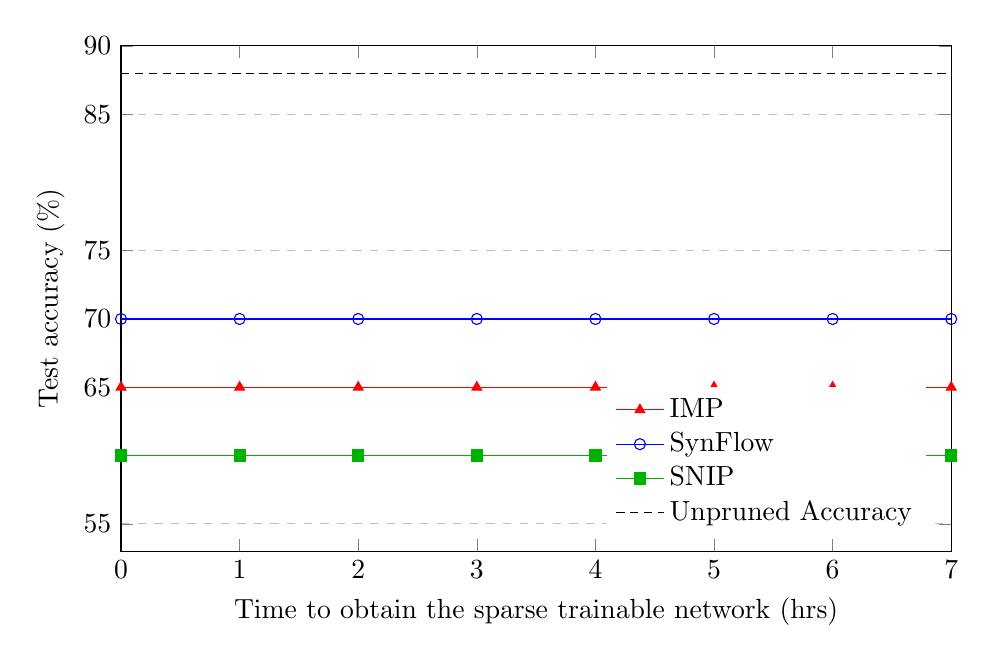
\begin{tikzpicture}
    \begin{axis}[
        width=\textwidth,
        height=8cm,
        xlabel={Time to obtain the sparse trainable network (hrs)},
        ylabel={Test accuracy (\%)},
        xmin=0, xmax=7,
        ymin=53, ymax=90,
        xtick={0,1,2,3,4,5,6,7},
        ytick={55,65,70,75,85,90},
        legend pos=south east,
        ymajorgrids=true,
        grid style=dashed,
        legend cell align=left,
        legend style={
            draw=none,
            /tikz/every even column/.append style={column sep=1em},
        },
        cycle list={
            red,mark=triangle*\\
            blue,mark=o\\
            green!70!black,mark=square*\\
            black,densely dashed\\
        }
    ]
    
    % Data series
    \addplot coordinates {(0,65) (1,65) (2,65) (3,65) (4,65) (5,65) (6,65) (7,65)};
    \addlegendentry{IMP}
    
    \addplot coordinates {(0,70) (1,70) (2,70) (3,70) (4,70) (5,70) (6,70) (7,70)};
    \addlegendentry{SynFlow}
    
    \addplot coordinates {(0,60) (1,60) (2,60) (3,60) (4,60) (5,60) (6,60) (7,60)};
    \addlegendentry{SNIP}
    
    \addplot coordinates {(0,88) (1,88) (2,88) (3,88) (4,88) (5,88) (6,88) (7,88)};
    \addlegendentry{Unpruned Accuracy}
    
    \end{axis}
\end{tikzpicture}

\end{document}